\documentclass{article}
\usepackage[utf8]{inputenc}
\usepackage{natbib}
\usepackage{booktabs}
\usepackage{graphicx}
\usepackage{subfig}
\usepackage{hyperref}
\usepackage{cleveref}
\graphicspath{ {./fig/} }
\title{Global, high resolution mapping of NO2}
\author{lu et al}
\date{April 2020}

\begin{document}

\maketitle

\abstract

High-resolution (100 m resolution or higher) mapping of NO2 provides opportunities to study the relationship between personal air pollution exposure and health over large populations and provide air pollution maps and human exposures with consistent uncertainties for global health studies. Statistical modelling of NO2 with geospatial predictors such as road density and meteorological variables may utilise ground station measurements at countries with a relatively dense monitoring network to provide an estimation for countries with deficient ground station measurements. We predict temporally-resolved NO2 world-wide at 25 m resolution, validate our product with external validations, and analyse the spatiotemporal dynamics of NO2. The global maps are provided at various spatiotemporal aggregations %(e.g. separating between weekdays and weekends, day and night) and spatial aggregations (e.g. multiple gridded resolutions, administrative units) 
to facilitate global exposure assessment. 

\section{Introduction}
Opportunities in global mapping of NO2, limitation in current studies. 
weekday and weekend, day, night: statistical predictive, exposure assessment

As NO2 varies considerably over time (e.g., between seasons), an annual estimation of NO2 and other air pollutants, as has been done in most of the classical LUR (land use regression) modeling \citep{Eeftens2012}, is unable to provide sufficient information to assess exposure when the space-time activities are considered. A relatively small number of studies developed models considering temporal variability of air pollutant concentration. \cite{BONIARDI2019108520} and \cite{CORDIOLI20171075} studying seasonal LUR models of Black carbon, PM$_x$, and common gaseous pollutants found considerable differences between warm and cold seasons.  \cite{rahman2017development} fit a LUR model to the residuals of a  periodic model of the day of the year and the day of the week to predict daily average  NO$_x$ concentrations. \cite{dons2013modeling} created a LUR model representing the diurnal cycle (hourly resolution) for Black Carbon. They developed different LUR models for each hour of the day, which has important implications in exposure studies.

Also, separation in time also affect the prediction patterns and accuracy in spatial mapping \citep{LU2020105856}.

 Evaluation of models includes uncertainty assessment as well as spatial validation methods. 
  

The objectives of this study are to: 
 \begin{enumerate}
\item develop a more in-depth understanding of the global modelling with external validation. 


\item provide an open-source, high resolution, temporally-resolved global NO2 dataset.

\item understand global NO2 patterns spatiotemporally. 
 
\end{enumerate}



 

\section{Method}


\subsection{Data}
This study is a considerable extension of the study \citep{LU2020105856} in terms of the measurement and predictor data collection. Specifically, we included the most comprehensive sets of official ground station measurements of European countries, Canada, United States, and Australia. In comparison, the station measurements of theses countries relied solely on the records from OpenAQ in \cite{LU2020105856}. This results in hourly NO2 measurements of 2017 from more than 7000 ground stations over the globe. The geospatial predictors are almost completed updated from \citep{LU2020105856}, the way of buffer calculation stays the same. Specifically, the differences are: 1) the OpenStreetMaps updated on 13 Apr 2020 is used to calculate the densities of roads and industrial areas; %The Sentinel-5 satellite (Tropomi instrument) annual column density measurements of 2018 is used. 
2) the wind strength and temperatures at 2 m altitude come from the ERA5-Land re-analysis model. 3) The elevation come from MERIT, 4) the population come from the GHS-POP R2019A. 5) The radiation is added; 6) the nightlight from the VIIRS re-sampled and aggregated over different buffers are added. All the predictors used are listed in \cref{tab-buff-pred} 
 

\begin{table*}\centering
\caption{Gridded predictors, data sources, and resolution.}
\label{tab-buff-pred}
\begin{tabular}{@{}lll@{}}\toprule
Variable&Source & resolution (nadir) \\ \midrule
 
elevation & MERIT DEM&  90m
radiation &?&	800m 
Wind and temperature & ERA5-Land &  9km
%        resolution	  nadir
%Temperature	0.1 degree	10km
%Wind 	    0.1 degree	10km
%population	0.0025 degree 	250m
%Night light	0.0042 degree	500m


\bottomrule
\end{tabular}
\end{table*}

 
\begin{table*}\centering
\caption{Buffered predictor variables and the buffer sizes}
\label{tab-buff-pred}
\begin{tabular}{@{}llll@{}}\toprule
variable & unit & original data type or resolution& buffersizes [m] \\ \midrule
roads 1 & m &LineString&25, 50, 100, 300, 500, 1000, 3000, 5000 \\
roads 2 & m& LineString&25, 50, 100, 300, 500, 1000, 3000, 5000 \\
roads 3 & m& LineString&25, 50, 100, 300, 500, 1000, 3000, 5000 \\
population  &? &250 m & 1000, 3000, 5000 \\
industry  & $m^2$&Polygon & 25, 50, 100, 300, 500, 1000, 3000, 5000\\
nightlight   & ?& 500 m& 450, 900, 3150, 4950\\
\bottomrule
\end{tabular}
\end{table*}

none-buffered: wind, temperature, tropomi, radiation, elevation.

\subsection{Data preprocessing}

%OLIVER
\subsection{Modelling}

 
\cite{LU2020105856} evaluated various statistical models including standard and regularised linear models and ensemble tree-based models and found the XGBoost model the most promising in global mapping. This study, the data is different, we compared again different models described in \cite{LU2020105856}

We chose XGB following...

A comparison is made with RF. 

XGB tuning

\subsection{Validation}

Accuracy matrix for weekday, weekend, day, night.

R2, RMSE, MAE, IQR

- Boostrapped CV

- Spatial cross-validation

Spatial-blocked CV,

Use Relative measures: 
R2, Relative RMSE (RMSE/median), for non-stationary NO2. 



 

\subsection{Mapping} 

\section{Result}
1. Validation result
cross validation, model interpretation, in appendix comparison with random forest
                   
2. Map
\begin{figure}
    \centering
    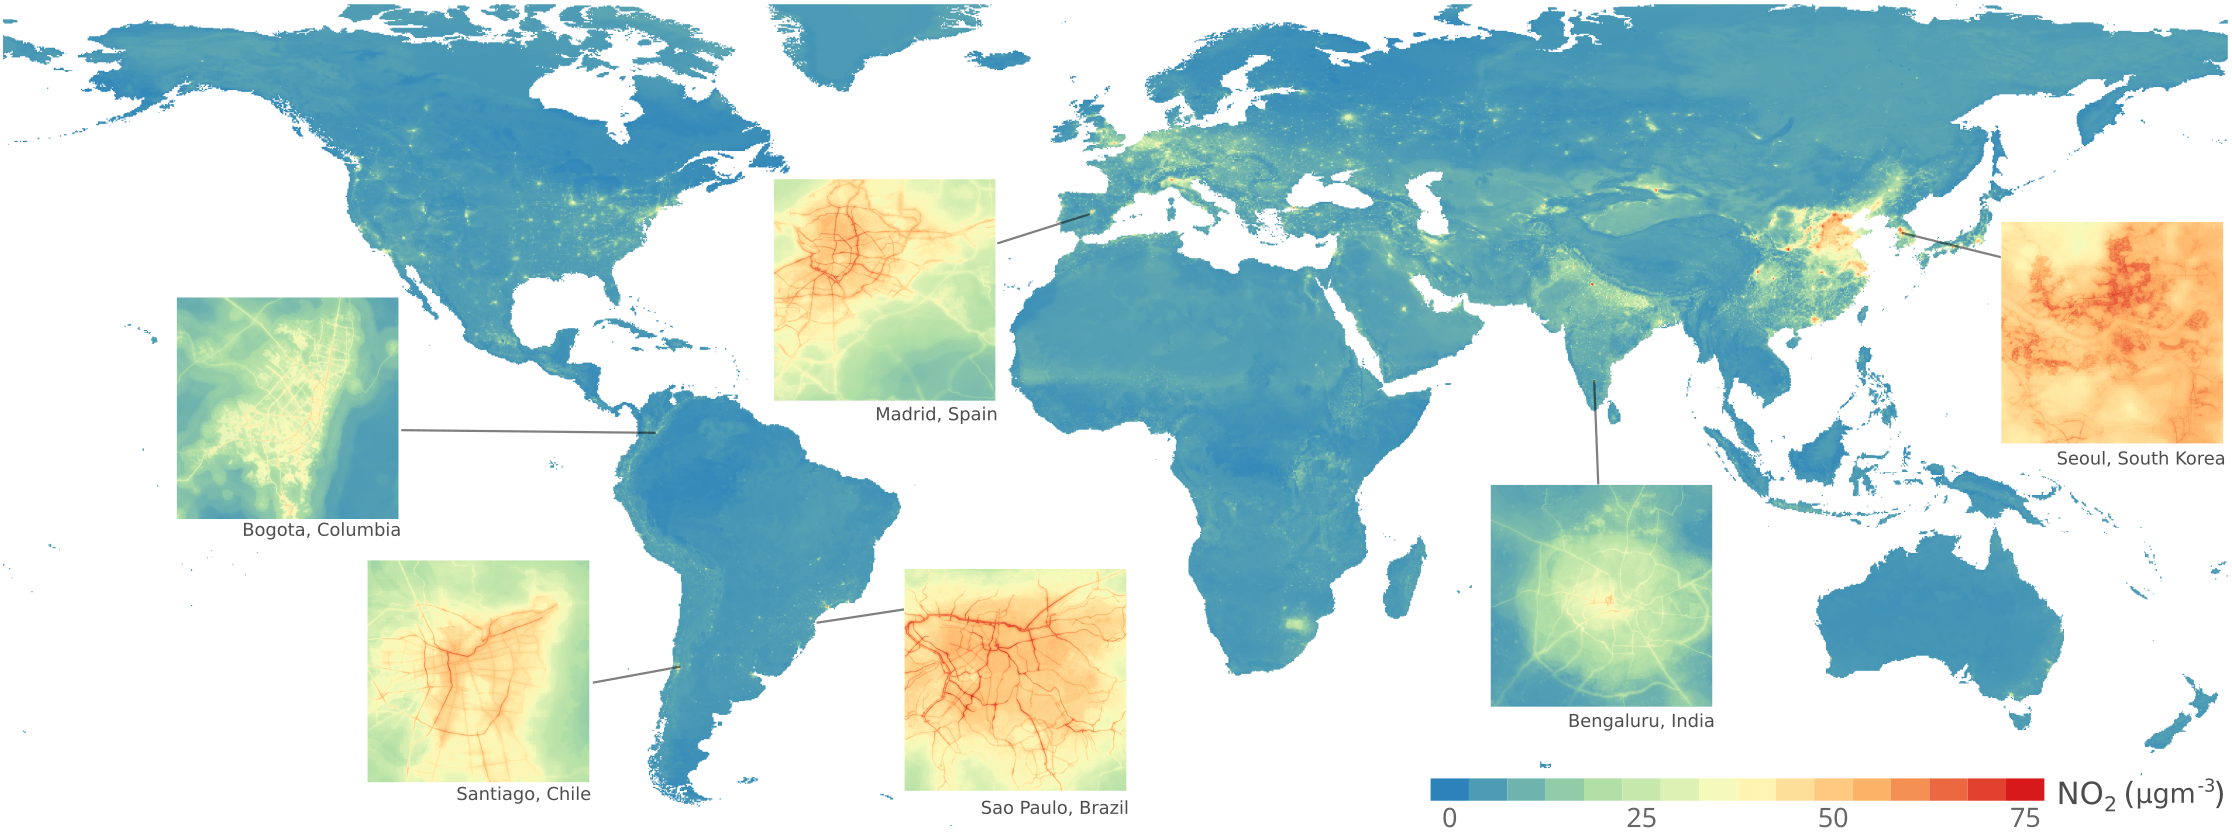
\includegraphics[width=\textwidth]{fig/glomap.png}
    \caption{global annual map, during daytime and in weekdays.}
    \label{fig:map}
\end{figure}

3. Spatial pattern in different temporal aggregations.

We show two examples in northern hemisphere and with relatively dense ground monitoring networks (\cref{fig:hamla}) and two examples in southern hemisphere and with relatively sparse ground monitoring networks (\cref{fig:adbo}). It can be observed that besides Los Angeles, USA, all examples show lower NO2 values at night times compared to the day times during weekdays. The Weekend daytime values are in general lower than the weekday daytime values. The night time values can be higher than the daytime values in some areas in weekends.   
 
\begin{figure}%
    \centering
    \subfloat[\centering Hamburg, Germany]{{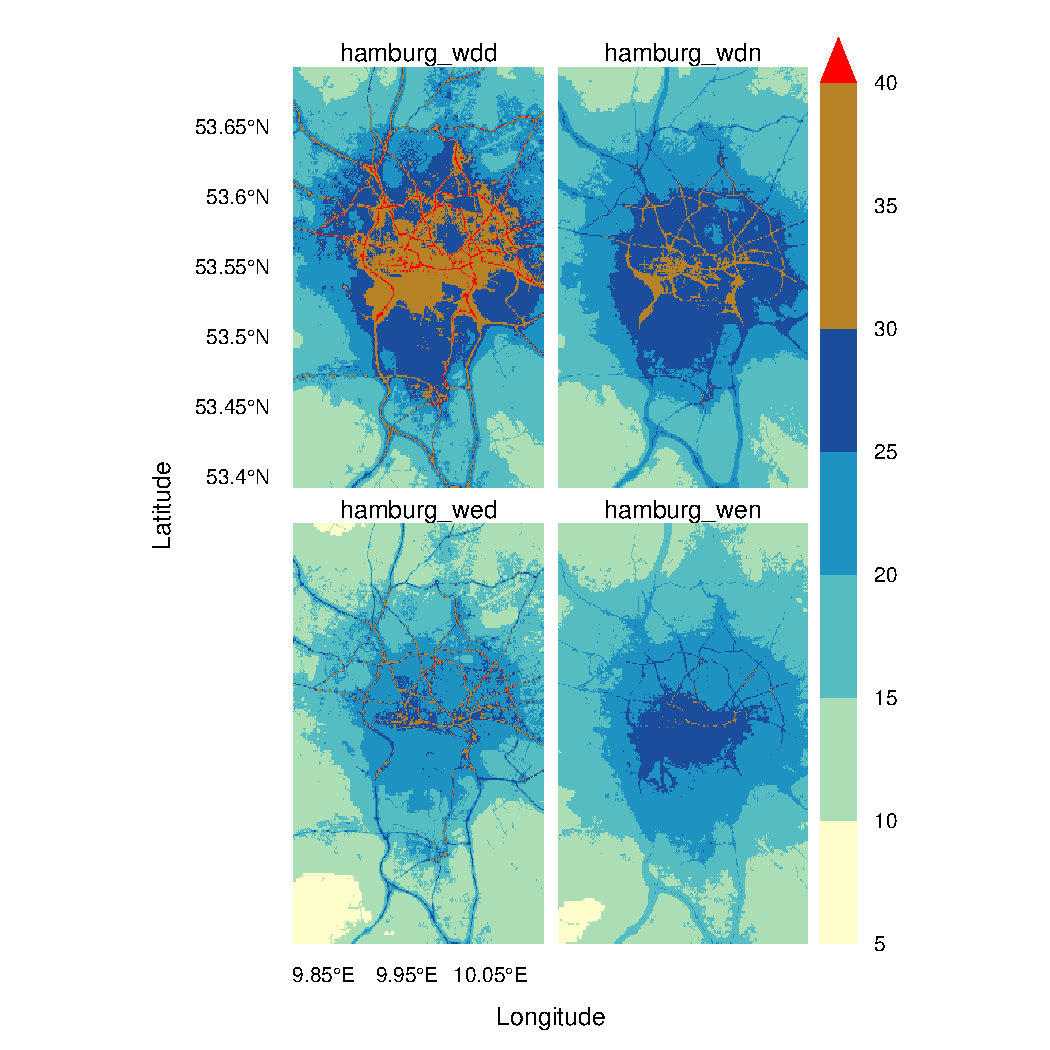
\includegraphics[width=5cm]{hamburg.pdf} }}%
    \qquad
    \subfloat[\centering Los Angeles, USA]{{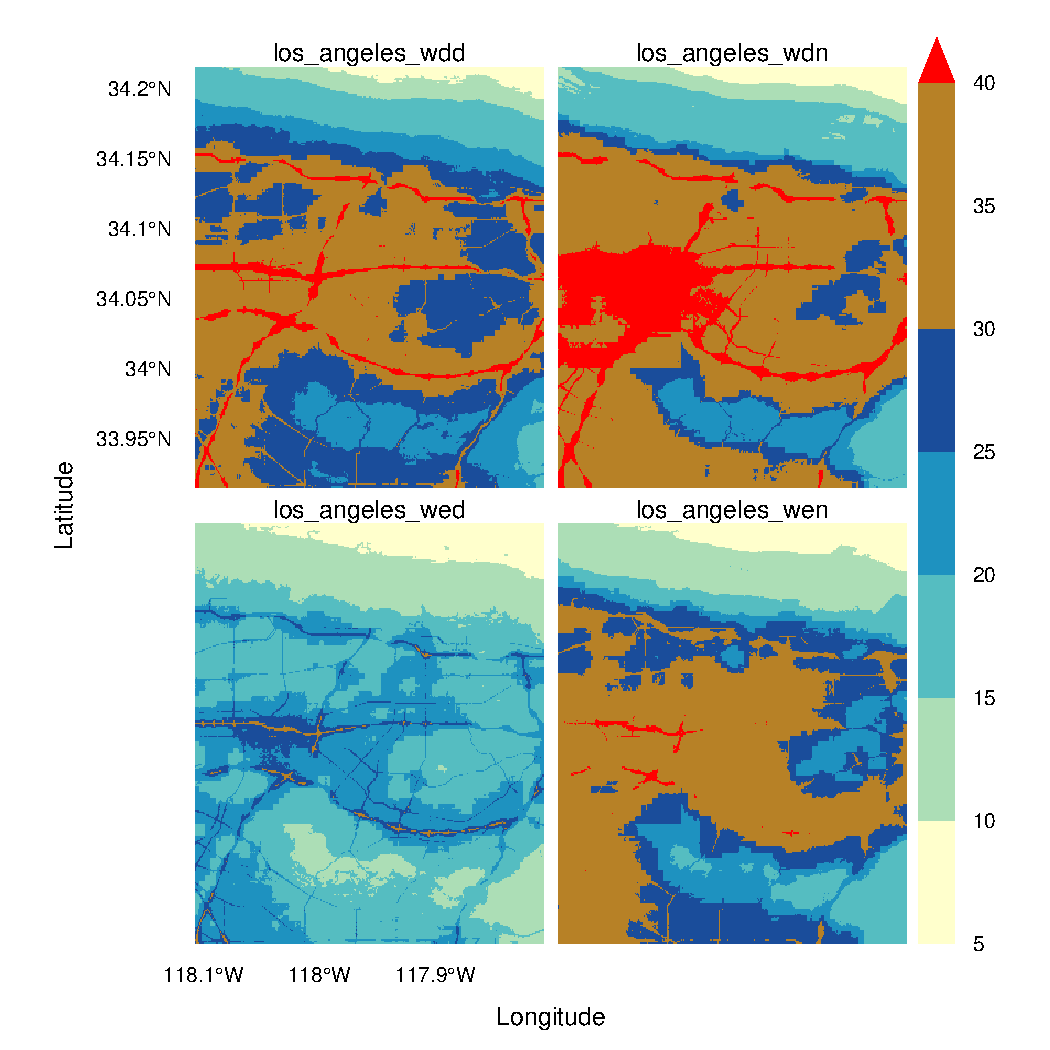
\includegraphics[width=5cm]{los_angeles.pdf} }}%
    \caption{Two examples in developed countries with relatively dense ground monitor networks.  wdd: weekday day, wdn: weekday night, wed: weekend day, wen: weekend night.}%
    \label{fig:hamla}%
\end{figure}

\begin{figure}%
    \centering
    \subfloat[\centering Addis Ababa, Euthopia]{{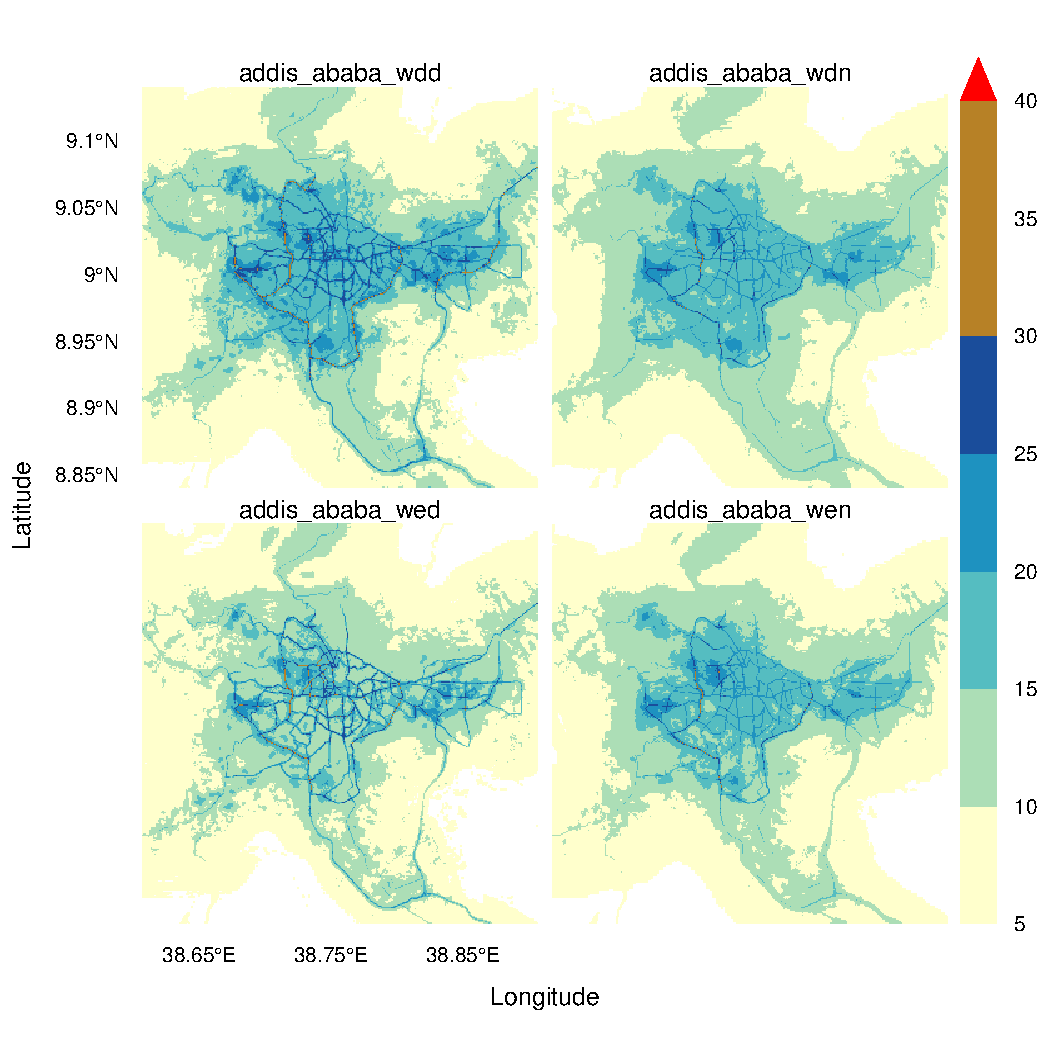
\includegraphics[width=5cm]{addis_ababa.pdf} }}%
    \qquad
    \subfloat[\centering Bogota, Columbia]{{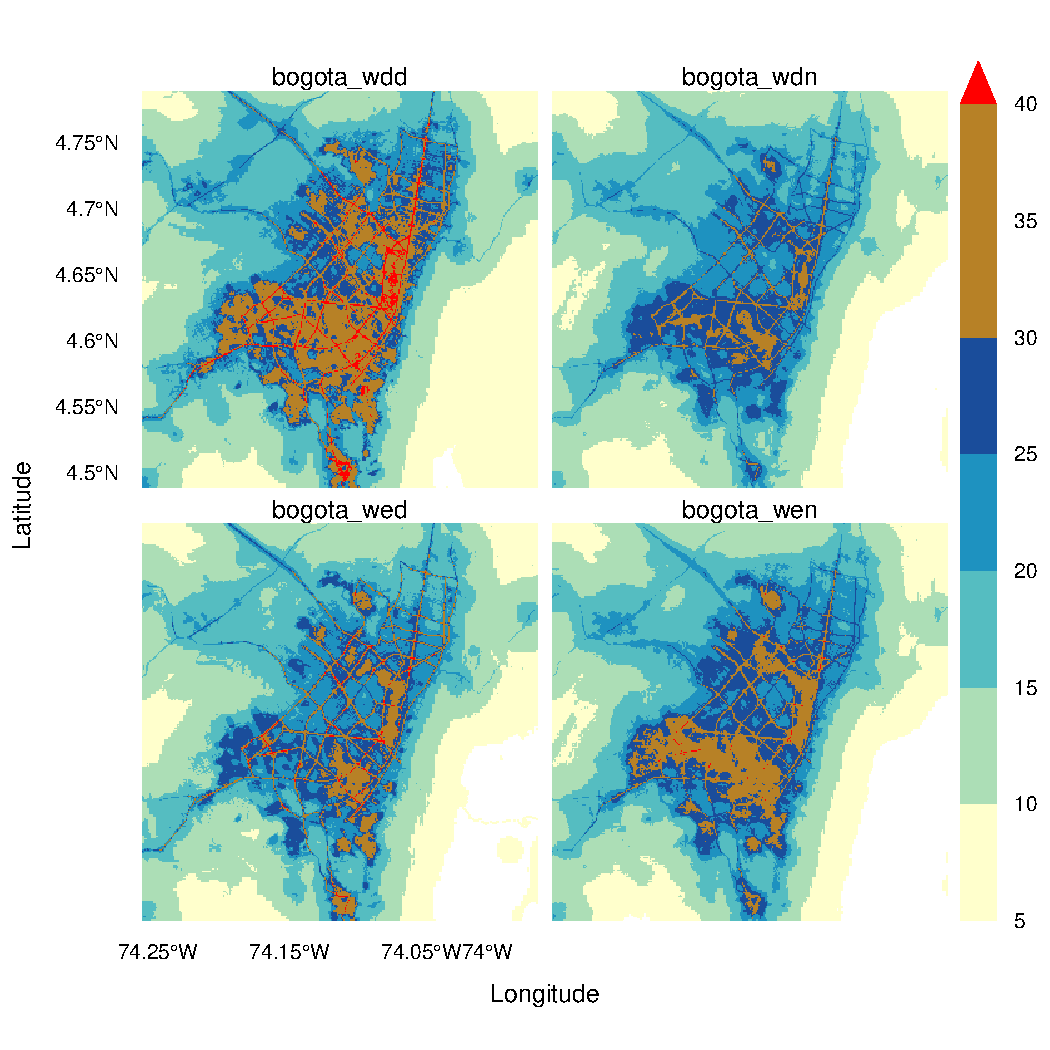
\includegraphics[width=5cm]{bogota.pdf} }}%
    \caption{Two examples in developing coutries with relatively sparse ground monitor networks.  wdd: weekday day, wdn: weekday night, wed: weekend day, wen: weekend night.}%
    \label{fig:adbo}%
\end{figure}

%4. Systematically select urban, suburban, industrial areas and compare their four temporal maps. 
4. Comparison between day, night, weekday, weekends through (normalised) substraction or division.

\begin{figure}
    \centering
    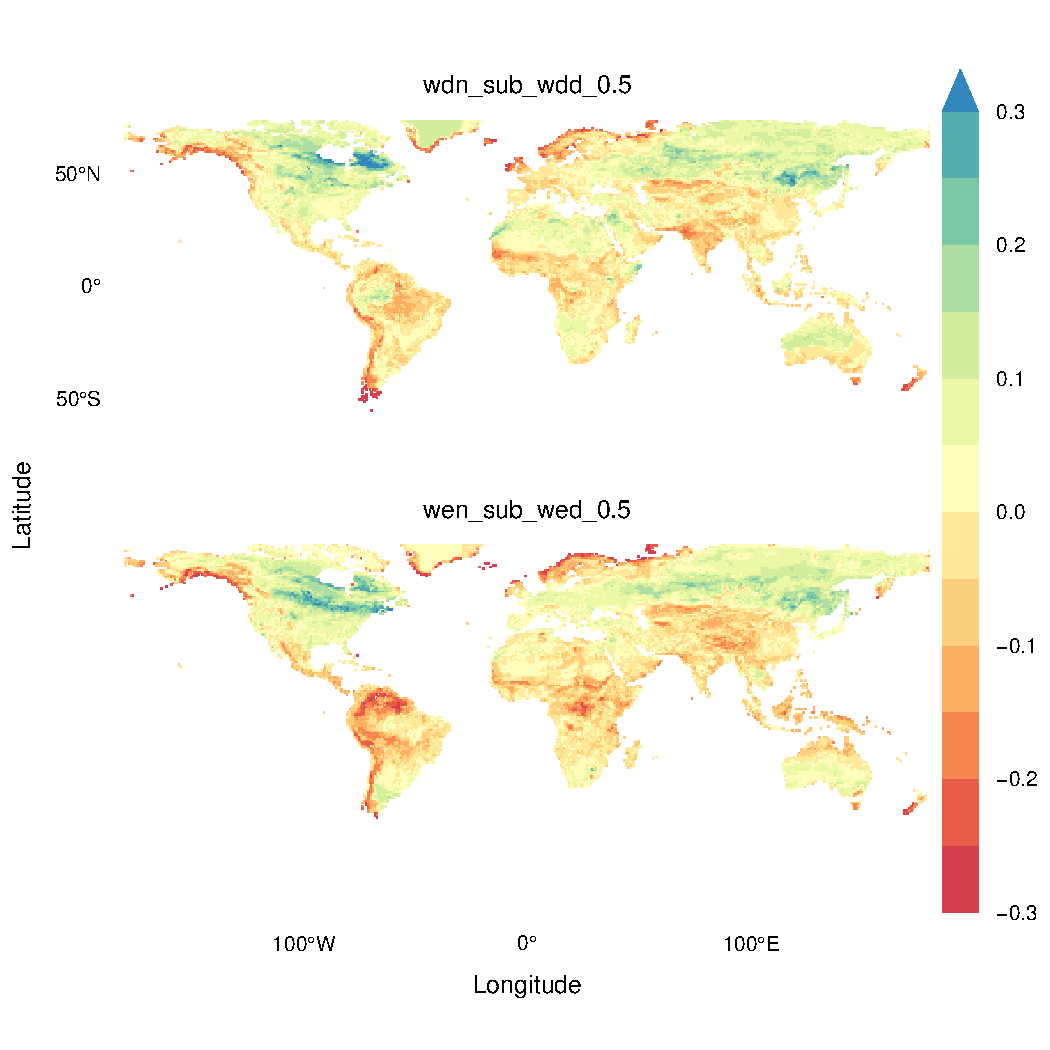
\includegraphics[scale=0.7]{fig/wen_sub_wed_0.5.pdf}
    \caption{differences between night and day, a: weekdays, b: weekends. "wdx" and "wex" indicates "week day" and "weekend"; "xxn" and "xxd" indicates "night" and "day", "0.5" indicates the results are up-sampled to 0.5 degree resolution for visualisation. }
    \label{fig:subdn}
\end{figure}

Observing \cref{fig:subdn}, we can summarise three patterns in terms of NO2 concentrations:

1) night$>$day for weekends but not weekday

This pattern may indicate lots of entertainment during night times in weekends and a relatively early rush hour after work.

Germany, Belgium, France, Spain, and the Netherlands show that in weekdays, NO2 concentrations are higher at daytime but in weekends at nighttime. The same pattern is shown along the western-southern coast of Australia, middle Brazil, southern America. 

2) night$>$day for weekday but not weekends
This pattern may indicate late work schedules, which result in late rush hours. 
Some areas, such as western China, eastern Peru and Western China, follow this pattern. 

3) nigh$>$day irregardless weekdays or weekends
As the radiation hinders the NO2 forming process, night $>$ day also occur in countries receiving high radiations during daytime. This theoretically happen to countries close to the equator. In this study, however, we observe this pattern in US, Canada except coastal areas, and Russia.  
The night>day NO2 may be caused by incomplete road networks and less populations. (observing the SHAP values for the four day and night models

5. map vs. tropomi 

Comparison with the mean in areas with dense ground station networks and with deficient measurements for comparison.



					
6, further validation: 
1)	Compare with other large-scale maps (ESCAPE or more recent maps)
2)	Other mobile sensing data, google car data? 


\section{Discussion}
Result discussion. 
Incompleteness OSM is a well-recognised issue and cannot be hidden. 

%question. where do we publish it, a web-service for viewing will greatly help with the publication. 
%The four maps in 10 km resolution with 100 m zoom in windows for details. 
%2.	On a map service, e.g. mapbox, publish the 4 maps
%3.	In a data depository, publish the predictors and 4 result maps (possibly 100m resolution)

In \cite{LU2020105856}, it was found that using an ensemble tree based algorithm, such as XGBoost \citep{chen2016xgboost}, the global model achieved a similar cross-validation accuracy in a country compared to the corresponding national models developed in countries with relatively densely distributed ground station networks. In comparison, a global linear regression model falls far behind those national models. On the one hand, it is a promising result showing that with machine learning methods, a global model could potentially catch up with the performance of a national model with relatively sufficient ground stations. On the other hand, the manuscript does not discuss the effect of unequal distribution of the ground stations in this analysis. The ground stations from countries with a relatively dense ground station network also dominate the global dataset and as a result, contributing the most to the NO2 process captured in a global model. As such, it might be too imprudent to claim that e.g. the XGB is promising in global modelling, though it is obviously outperform a linear regression model, at least with the current data availability. 


\section{Conclusion}


\bibliographystyle{plain}
\bibliography{ref.bib}
 \section{To be clarified}

 1. the area (extent) of the world.   
 2. computation time
 3. all data convert back to wgs84 (4626) before merging?
 - gdal\_merge requires the same CRS for datasets to be merged. 
- we could consider to merge to 6x6 degree and publish those, similar approach is done by others
- how to publish data? (zenodo etc); creating a viewer and host?

\end{document}

\urlhttps{https://ngdc.noaa.gov/eog/viirs/download_dnb_composites.html} nightlight, 6 tiles, 2016 annual is available. 



\section{Tasks and time schedule}

Night light of 2017, monthly
NOAA/NCEI - Earth Observation Group - Defense Meteorological Satellite Progam, Boulder
"vcm-orm-ntl"
\urlhttps{https://ngdc.noaa.gov/eog/viirs/download_dnb_composites.html}

some minor updates for tomorrow based on the document and manuscript:
\begin{verbatim}
 
-M: overlap needed - all data convert back to wgs84 4626 before merging
-M: climate data has lots of missing data

\end{verbatim}
